
%
%  $Description: Author guidelines and sample document in LaTeX 2.09$ 
%
%  $Author: ienne $
%  $Date: 1995/09/15 15:20:59 $
%  $Revision: 1.4 $
%

\documentclass[times, 10pt,twocolumn]{article} 
\usepackage{latex8}
\usepackage{times}
\usepackage{graphicx}
\usepackage{subcaption}

%\documentstyle[times,art10,twocolumn,latex8]{article}

%------------------------------------------------------------------------- 
% take the % away on next line to produce the final camera-ready version 
\pagestyle{empty}

%------------------------------------------------------------------------- 
\begin{document}

% \title{Epidemics Graph Neural Network Node Classification}
\title{Epidemics Graph Neural Network Node Classification and Link Prediction}

\author{Jaykumar Patel\\
patel.jay4802@utexas.edu\\
% For a paper whose authors are all at the same institution, 
% omit the following lines up until the closing ``}''.
% Additional authors and addresses can be added with ``\and'', 
% just like the second author.
\and
Afnan Mir\\
afnanmir@utexas.edu\\
}

\maketitle
\thispagestyle{empty}

\begin{abstract}
The COVID-19 pandemic has shown that contact tracing is a key way to mitigate the spread of the disease. However, manual contact tracing is slow and can be inaccurate. Thus, this project aims to automate contact tracing by utilizing Graph Neural Networks (GNNs). In our preliminary work on network analysis and simluations, we found that the contact network is a combination of an exponential and scale-free network, and an infection starts spreading slowly, but with some time, the rate of infection increases rapidly. 
\end{abstract}


%------------------------------------------------------------------------- 
\Section{Introduction and Motivation}

When COVID-19 first appeared, a key way that its spread was mitigated was through contact tracing. Contact tracing is the process of tracking how the virus spread by identifying people who may have come in contact with an infected person.

However, the pandemic revealed that the COVID-19 disease can spread faster than manual contact tracing. Thus, the objective of this project is to automate contact tracing by incorporating machine learning using GNNs, which will allow quicker contact tracing, and possibly lead to a greater mitigation of the spread of COVID-19 when compared to manual contact tracing.

% - What is the big picture? What is the main objective of this project?
% - Why is this project interesting?

%------------------------------------------------------------------------- 

\Section{Previous Work}
Methods pertaining to predicting the spread of COVID-19 include mathematical models, traditional ML models, and graph-based ML models. 

One example of a mathematical model is the SEIRD model, which attempts to predict the change in Susceptible, Exposed, Infected, Recovered, and Deceased people over time through the use of differential equations. This model is used to simulate the spread of the virus over time \cite{SEIRD-LSTM}.
% (https://www.frontiersin.org/articles/10.3389/fpubh.2021.727274/full)
SIR is simpler version of the SIERD model, which attempts to perform the same task \cite{SIR}.
% https://www.medrxiv.org/content/10.1101/2020.05.15.20103077v2

Traditional ML models have also been used to predict the spread of COVID-19. For example, Long Short-Term Memory (LSTM) models have been used to predict the number of cases over time \cite{SEIRD-LSTM}. 
% https://www.frontiersin.org/articles/10.3389/fpubh.2021.727274/full
Another approach utilizes a hybrid of SIRD and LSTM to account for time dependent parameters of the SIRD model \cite{SIRD-LSTM-hybrid}.
% https://www.nature.com/articles/s41598-022-06992-0

Furthermore, graph-based ML models, such as GNNs, have been used on mobility data to predict the number of cases and hospitalizations \cite{positivity-hospitalization-GNN}.
% https://www.ncbi.nlm.nih.gov/pmc/articles/PMC10066232/#:~:text=Message%20passing%20instances%20of%20GNNs,as%20well%20as%20hospitalization%20rates.
GNNs can also be used for link prediction, which is useful for contact tracing \cite{contact-tracing-GNN}\cite{link-prediction-GNN}. 
% https://proceedings.neurips.cc/paper_files/paper/2018/file/53f0d7c537d99b3824f0f99d62ea2428-Paper.pdf

% Feature Based Approach:
%     - Multivariate Logistic Regression to predict infectious risk
%     - Might not be an actual study, just a proposal
% https://www.ncbi.nlm.nih.gov/pmc/articles/PMC8570232/#Sec2title


% https://www.frontiersin.org/articles/10.3389/fpubh.2021.727274/full
% Uses 2 approaches:
% SEIRD - Susceptible, Exposed, Infectious, Recovered, Deceased
%     - simulating the spread of the virus over time
%     - Simulation Approach
% LSTM
%     - To predict the number of cases over time by training the NN over a subset of time
%     - ML Approach

% Previously used methods for predicting infections include mathemical models and ML models.
% One example of a mathemical model is the SEIRD model, which attempts to predict the change in Susceptible, Exposed, Infected, Recovered, and Deceased people over time through the use of differential equations. This model is used to simulate the spread of the virus over time. 

% https://www.ncbi.nlm.nih.gov/pmc/articles/PMC10066232/#:~:text=Message%20passing%20instances%20of%20GNNs,as%20well%20as%20hospitalization%20rates.
%     - utilizes GNNs on mobility data to predict number of cases and hospitalizations


% https://www.nature.com/articles/s41598-021-97037-5
%     - Combined mathemical and ML models
%     - Specifically uses LSTM to predict number of cases over time
%     - Uses Markov Model to reduce prediction error of the LSTM

% https://www.nature.com/articles/s41598-022-06992-0
%     - Combines LSTM and SIRD
%     - Uses LSTM to solve for the time dependent parameters of the SIRD model
%     - Uses LSTM to predict the number of cases over time









\Section{Approach}

We used the foursquare dataset to build a contact tracing graph of Austin, Texas \cite{DVN/PFLAH4_2020}. Each entry contains data such as a unique device ID, a location ID, UTC date and hour, and a dwell time, which all tell us when a person visited a location and for how much time. Given this data, we generated a contact tracing graph for people in Austin.

We used data only from July 1st, 2020 to generate a sample network. Our nodes were all the unique device IDs in the dataset. For our edges, we used the following logic: we ignored entries whose dwell time was less than 60 minutes, as we assumed less than an hour was not enough time to make significant contact with others. Then, we used the UTC date and hour with the dwell time to determine an arrival and departure time for each entry. We then compared every entry with every other entry and checked if there was any overlap between their dwelling times. If there was, we considered this as a contact between the two people. We then added an edge between the two people in our graph.

In addition, we created a sample Susceptible-Infected simulation using the dataset. We did not include a recovery/death or incubation period in this simulation model mainly because we only performed the simulation over one day. To perform the simulation, we did the following: We randomly selected 20\% of the nodes in the graph to be infected. Next, with each time step (1 hour), we looked at all the neighbors of each infected node and infected them with a probability of 1.0, so we assumed any contact led to an infection. We did this for a 24 hour time range.


\Section{Experimental Setup and Results}
In Figure \ref{fig:my_label}, we can see the contact network after one day.
\begin{figure}
    \centering
    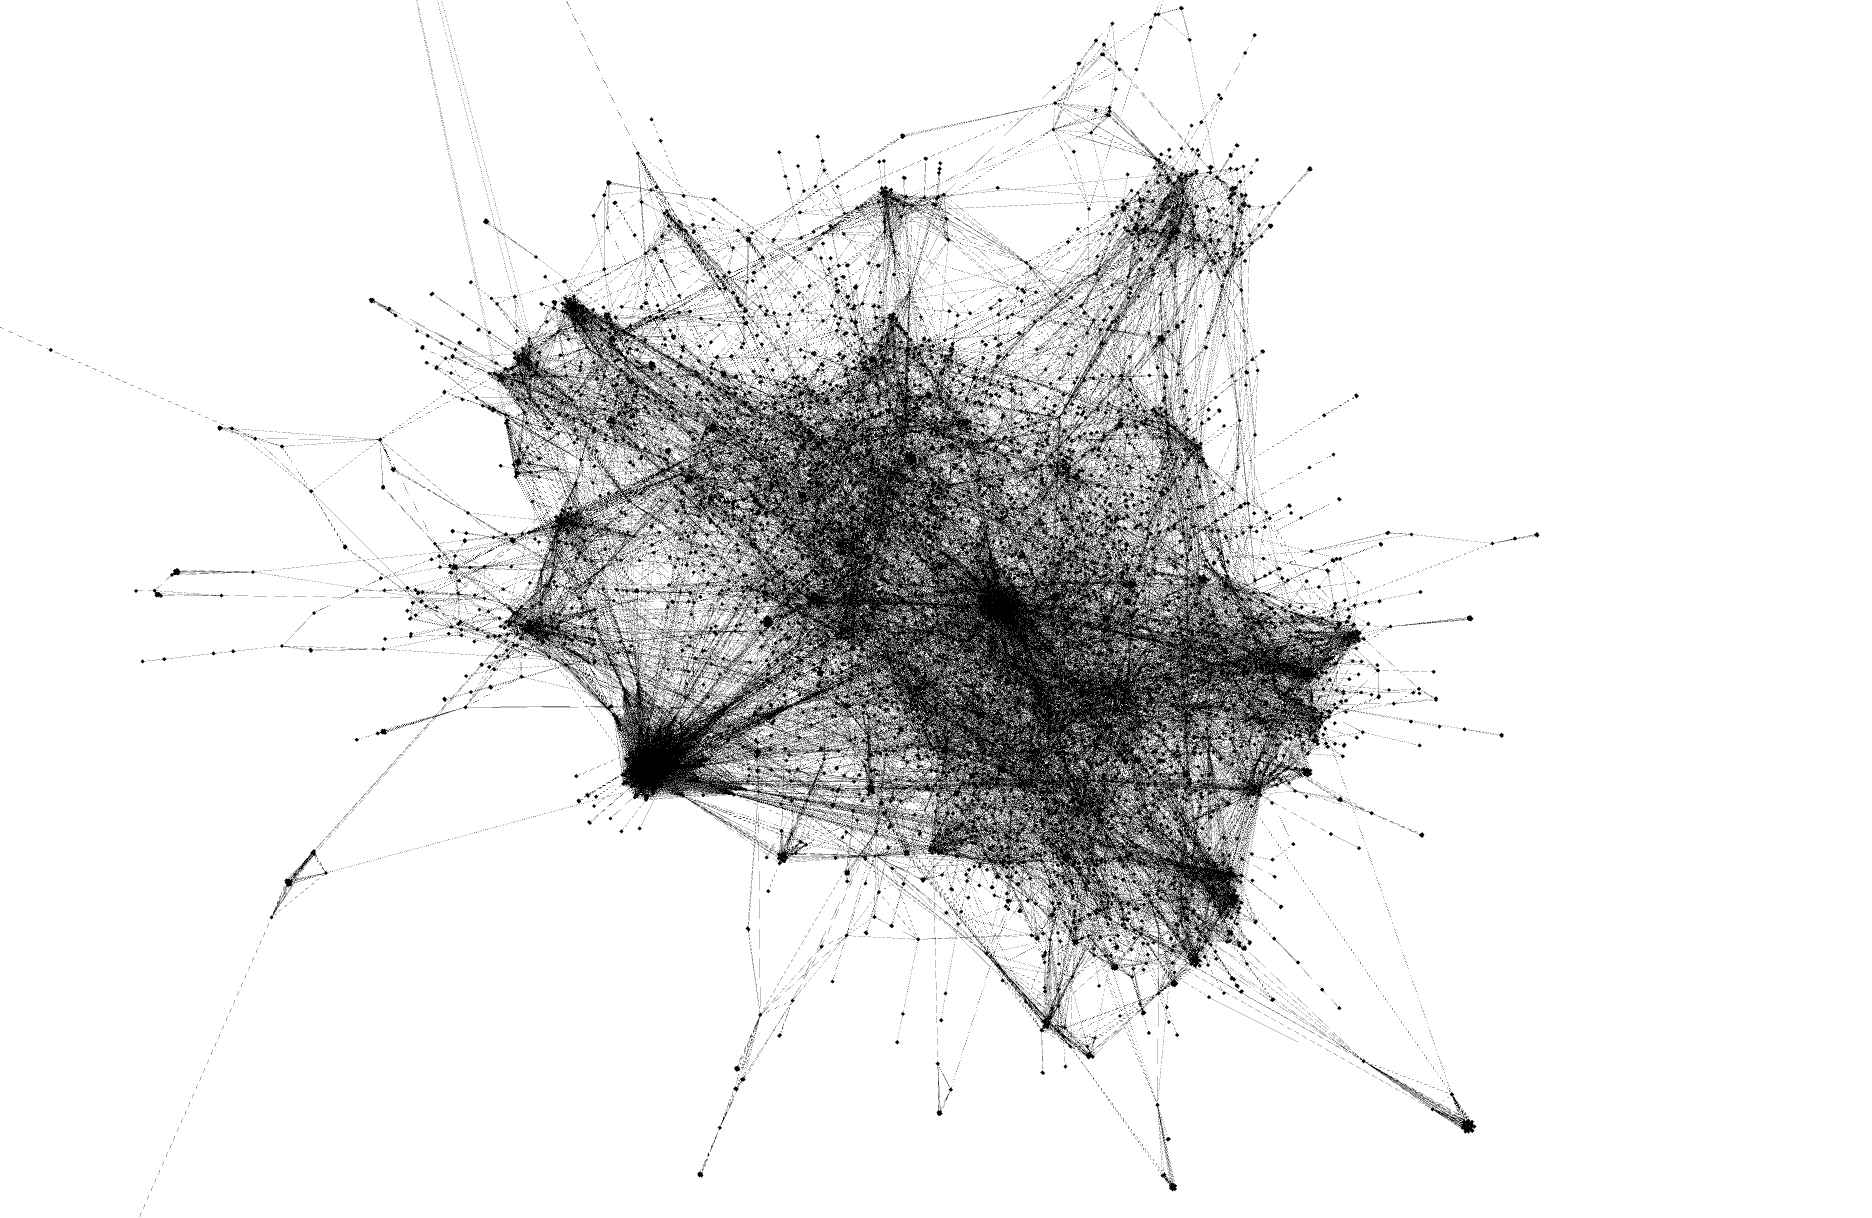
\includegraphics[width=0.30\textwidth]{imgs/one_day_net.png}
    \caption{Network after one day}
    \label{fig:my_label}
\end{figure}
Network properties for this network were also calculated. The average node degree is 10.41, the network diameter is 14, the average clustering coefficient is 0.687, and the average path length is 4.784. In addition to this, the degree distribution was mainly an exponential distribution with subtle hints at a power-law. This can also be seen from the network itself, as we can see the presence of a few hubs in the network. This makes sense, as we should expect a social network to be scale-free, but we do not have all the data points, so it is not fully scale-free on the sample network.

In addition, we can see the resulting infected graph from our simulation in Figure \ref{fig:my_label2}.
\begin{figure}
    \centering
    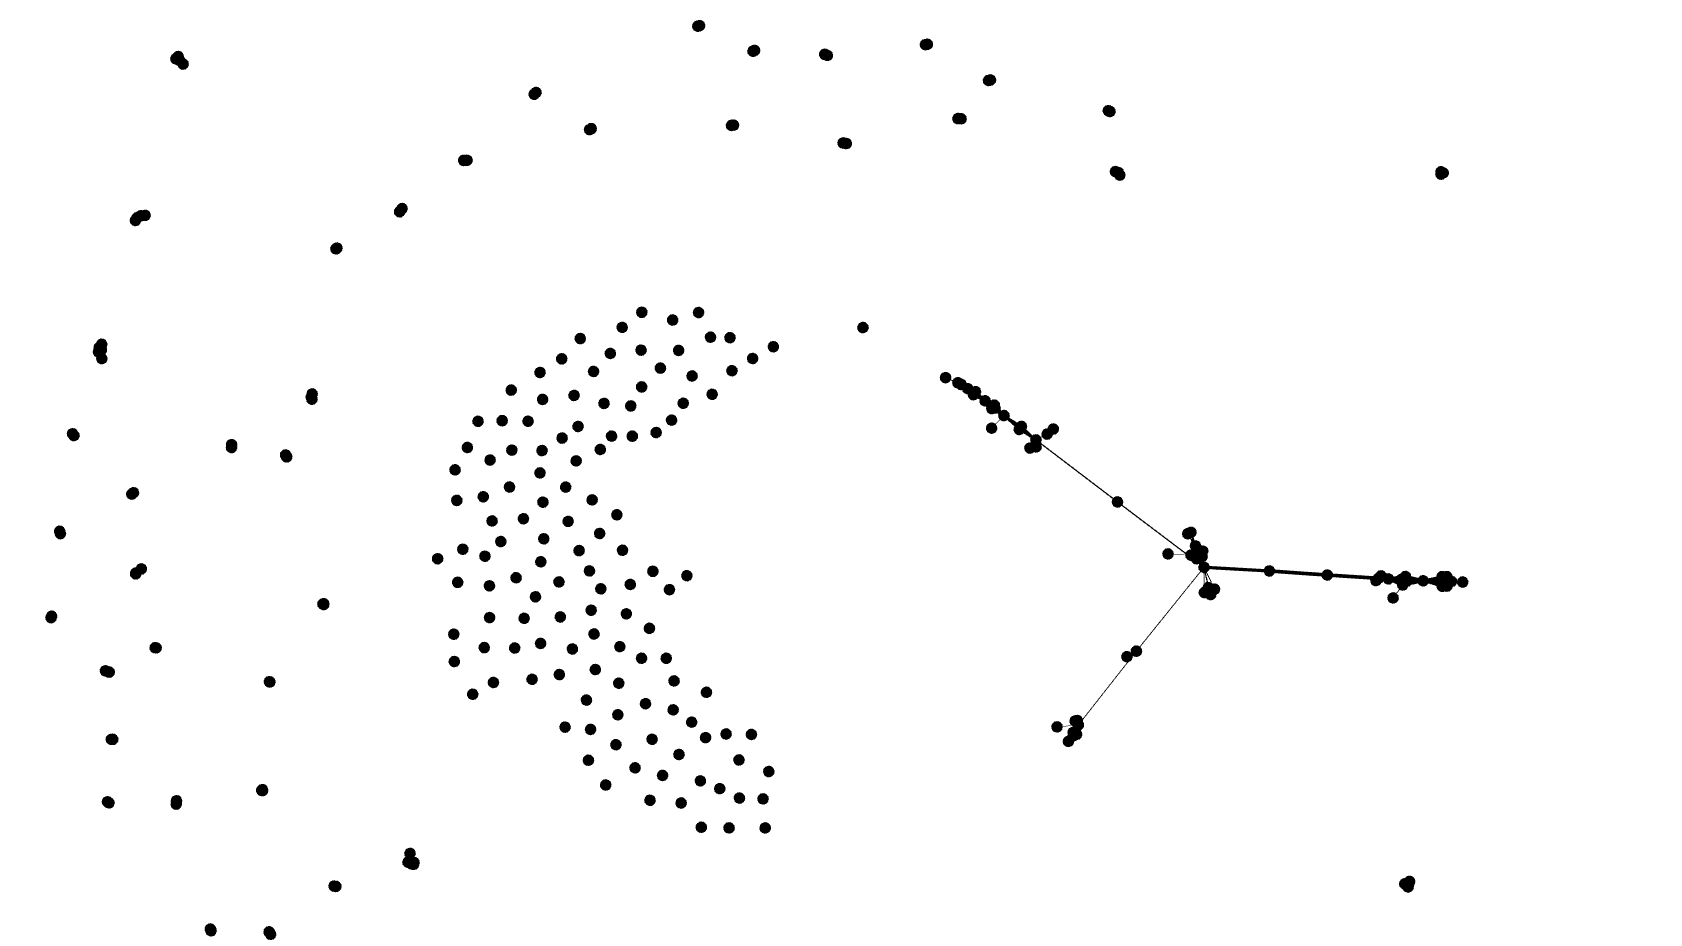
\includegraphics[width=0.30\textwidth]{imgs/simulation.png}
    \caption{Infected graph after one day}
    \label{fig:my_label2}
\end{figure}
In this network, it is important to note that all of the visible nodes are infected, and the edges represent how the infection has been spread. We can see that not a lot of infected nodes have spread the disease, but the ones that have created one connected component that show the beginnings of a scale-free network. 

In Figure \ref{fig:my_label3}, we can see the number of infected nodes over time. We can see that the infection doesn't really start to spread until the latter half of the day, and then looks as though the rate of infection is about to increase exponentially before the day ends. This lines up with our intuition, as we would expect the infection to spread faster as more people get infected.
\begin{figure}
    \centering
    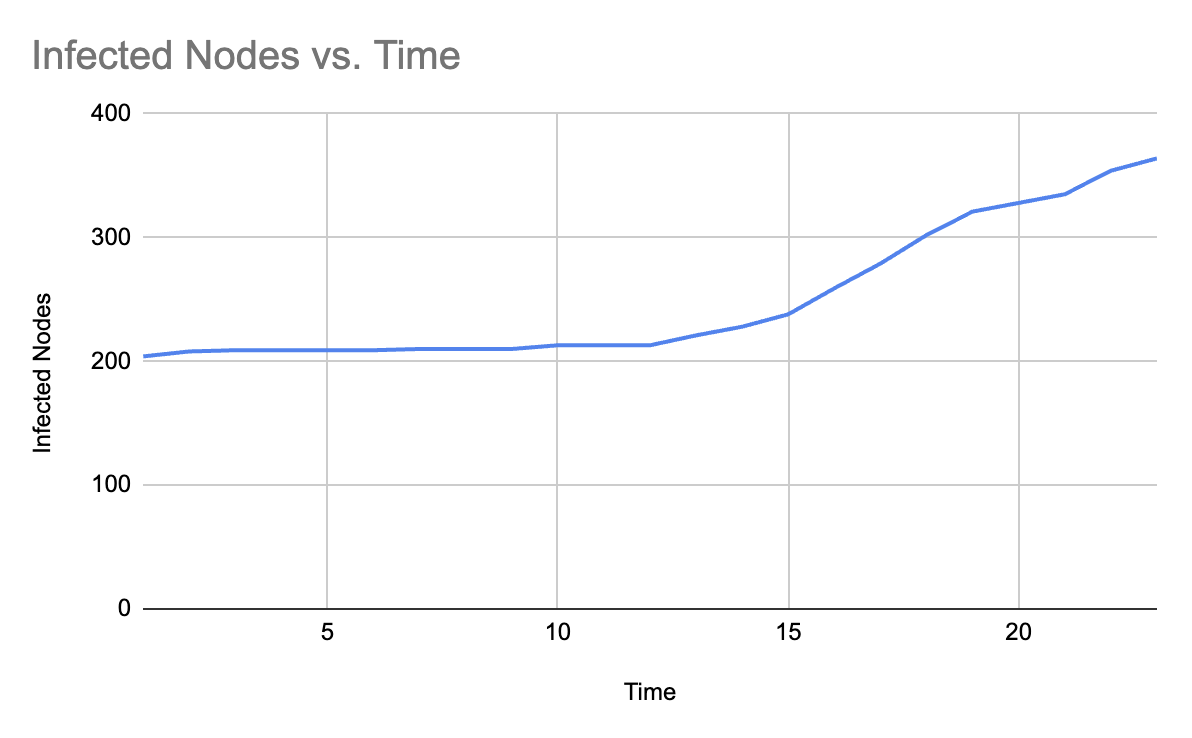
\includegraphics[width=0.30\textwidth]{imgs/infected_over_time.png}
    \caption{Number of infected nodes over time}
    \label{fig:my_label3}
\end{figure}


\Section{Conclusion and Short-Term Plans}
Through the analysis of the network, we were able to determine the network of contacts is a combination of an exponential and scale-free network. Some people came into contact with many other people where as others stayed within their cliques. The simulation showed that the virus initially spread slowly, but the rate of infection increased rapidly. As people with many connections became infected, the virus was able to spread significantly faster.


For M2, we plan to do a more complete analysis of the network by considering both July and August data. We also plan to run more simulations. Specifically, we want to make them more realistic by accounting for the incubation period, deaths from the virus, and the fact that people may not be able to get infected again after they have recovered. We also plan to implement GNNs at a small scale to perform link prediction. Specifically, we will use GNNs to predict the people that come into contact with previously infected people. By predicting contact between people, we will be able to predict the spread of the virus.

%------------------------------------------------------------------------- 
% \Section{Objectives and Deliverables}

% First, we will analyze the networks to determine their properties. Then, to better understand network behavior, we will run simulation to see how COVID-19 spreads through the network.

% The main goal of contact tracing is to find people who may be infected due to their contact with other infected people. Similarly, this project will aim to classify infected nodes in a graph, where nodes represent people, and links represent contact between people. This network will be formed by utilizing real contact information from mobile devices. In order to predict infections within a network, this project will implement and analyze GNNs, specifically link prediction. 

% The dataset we will be using is the ``foursquare'' mobility dataset that consists of location visit logs in Austin, TX from 2019 to 2021. The visit log includes information about when and where a device was, as well as how long it was there. 
% - What are the main research questions you plan to address?
% - How exactly is the “network” formed? What is a “node” and what is a “link”?
% - Which dataset(s) do you plan to use?
% - What are the deliverables?

%------------------------------------------------------------------------- 
% \Section{Tasks and Timeline}

% Firstly, we will collect and clean the data. This includes reformatting and filtering the data. We will analyze the dataset to get a better understanding of its properties (such as degree, betweenness centrality, clustering coefficient, etc.). We plan to complete this by October 10th, 2023.

% Then we plan to run simulations on the network to get a better understand of how the virus flows. We plan to complete this by November 14th, 2023.

% Finally, we will utilize GNNs to perform link prediction to see how the network evolves over time. We plan to complete this by November 30th, 2023.

% We will pair program; thus, the member contribution will be 50/50.

% - What are the main tasks of your project?
% - What is the proposed timeline (w.r.t. project milestones) and member(s) contribution?

%------------------------------------------------------------------------- 

% \Section{Conclusion and References}

% In conclusion, the project aims to utilize GNNs to make contact tracing more efficient and accurate. We will analyze the dataset to understand its properties, we will run simulations to see how the virus spreads through the network, and we will train GNNs to perform link prediction.

% We will start by researching GNNs. Particularly, we will look at an article by Neptune.ai on the application of GNNs and a DGL tutorial on link prediction \cite{menzli-blog} \cite{dglLinkPrediction}.

% https://towardsdatascience.com/graph-convolutional-networks-introduction-to-gnns-24b3f60d6c95
% https://neptune.ai/blog/graph-neural-network-and-some-of-gnn-applications#:~:text=Graph%20Neural%20Networks%20(GNNs)%20are,and%20graph%2Dlevel%20prediction%20tasks.
% https://docs.dgl.ai/en/0.8.x/tutorials/blitz/4_link_predict.html

% what a GNNs is, and how to use it (blogs on this).

% - Briefly summarize the project idea and main contributions.
% - Include some starting points (e.g., papers, websites, datasets, etc., preferably more than what
% was given to you as a starting point in the projects description).


%------------------------------------------------------------------------- 
% \nocite{ex1,ex2}
\bibliographystyle{latex8}
\bibliography{latex8}

\end{document}

